\chapter{Application}\label{chap:application}
In order to create a robust system, two solutions are proposed. The first utilizes the fact that a person faces 
the same direction their waist faces. So we create a plane between three fixed 
points, the center hip $\vec{c}$, the left $\vec{l}$ and the right hips $\vec{r}$. A normal vector \N was created 
from this plane in order to allow the program to recognize where the person is 
facing.

\begin{figure}[!htbp]
\centering
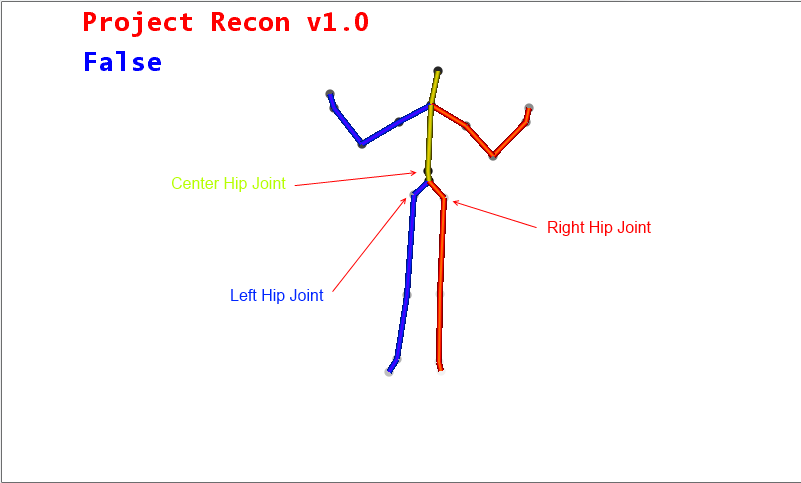
\includegraphics[width=1\textwidth]{images/skeleton_frame3.png}
\caption{In the figure the three joints are pointed out and named}
\label{skeletonframe3}
\end{figure}

To calculate the normal vector, we subtract the right and left hip joints from 
the center hip joint and then we calculate the cross product of the two 
subtractions.

$\vec{N}$ = ($\vec{r}$ - $\vec{c}$) $\times$ ($\vec{l}$ - $\vec{c}$)

We then calculate the normal by using the Normalize method.

\begin{verbatim}
var dir = Vector3.Cross(rhip - chip, lhip - chip);
var norm = Vector3.Normalize(dir);
\end{verbatim}

As the person turns, the normal vector will be used as a reference to calculate the angle between it and the Z axis. This will allow us to rotate the skeleton so that it will be always facing the Kinect. Recognition will then take place.

Kinect has another problem, which is that it cannot diffrentiate between a user giving it his face or his back. In other words, a user's left and right are swaped if the user is giving the Kinect his back.

%put an image to make it better understandable

The normal vector calculation approach will reswap the left joints with the right joints when the \N is on the negative Z axis. 
However, here another problem emerges. When the swap takes place, an error occurs. Mainly, the programmer can not 
edit the value of the position of the joints. The value is read from the skeleton 
stream of the Kinect. In order to resolve this, an avatar skeleton needs to be 
created, littleGuy. littleGuy is an array of SkeletonPoints, where every 
SkeletonPoint represents a joint, and gets the value from these joints. This 
helps in allowing us to edit and the SkeletonPoints as we wish and in the end 
draw this avatar skeleton instead.

In figure~\ref{skeletonnormal} the user is facing their right, having the normal vector (red 
line) erected and defining the direction the user is facing.

\begin{figure}[!htbp]
\centering
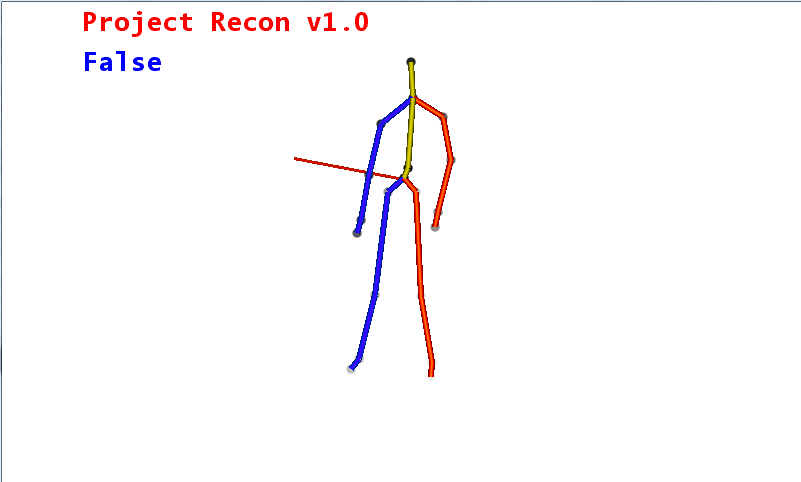
\includegraphics[width=1\textwidth]{images/skeleton_normal.png}
\caption{Skeleton with a normal vector defining where it is facing}
\label{skeletonnormal}
\end{figure}

The translation and rotation of the skeleton occurs in the Skeleton Space. The algorithm translates littleGuy to the origin point where it calculates the \N. Rotation occurs in the origin and then the new manipulated littleGuy translates back to a fixed point in the Z axis, the Y axis and X axis however remain in the origin. After this Project Recon stores the translated littleGuy in a new avatar skeleton called transGuy. The program then renders transGuy to the 2D Color Space. 

The second step is using Kinect's face detection capabilities, which may be 
hard and require high processing. Errors may occur when Kinect re-swaps the joints to their right place. For this we will use the face dectetion capabilities of Kinect to create a sanity check. That is if the swap did occur and the user's face was visible, then the swap is a mistake and it will re-swap again to the correct state.

When it came to testing the normalization of the skeleton using the Kinect, a problem emerges. When the user has a joint not facing the Kinect, then the Kinect does not have the position value of this joint. The reason for this is that no infrared rays are reflected from this joint. In turn, when the rotation occurs the some joints have false space(X, Y, and Z) values. This error will question the validity of the rendered and final translated values of the joints. This error made us discard this method and resort to a different one that will also aims to maintain the robustness of the system.

%here talk about the final way and discuss how you will use the recognition to solve the issue with robustness 
\section{Recognition}
Recognition is the essence of this project. Recognition needs to be in real time, but most importantly how will the recognition occur. We discussed in the previous section the resolve of the normal vector. However, why is it needed? In recognition we want to be able to translate the skeleton of the person in order to always recognize from the same direction, facing the Kinect. In the coming sections we will discuss the different ways for recognition.

\subsection{Glyphs Method}
This is the proposed method in the case of recognition taking place after rotation by the help of \N as discussed earlier in this chapter. The idea behind it is to create a path taken by each joint from the skeleton and store it in an image. Creating a single image with the overall motion is and comparing it with the reference image, would be more optimal than taking a number of frames and comparing them with other reference frames.

As a joint moves, it creates a path shadowing its past movements. Each joint has its own exclusive color in order to differentiate if lines intersect. When the user moves the system will draw the paths taken by the joints creating some sort of a glyph image depicting the overall motion of the skeleton. An example of how a glyph would like is in both figures below. Figure 1 shows the user as he executes a move with each joint creating a path. Figure 2 shows the final glyph as it would be stored.

%image of a person with a glyph
%image with a glyph

After storing the glyph image, a process of image processing would take place where comparisons between the captured glyph image and the reference glyph images would begin. When a match is found, the technique would be recognized, if a match was not found the glyph image is discarded. Recognition when comparing two glyph images would of course have some sort of threshold as users are different in their executions of a technique.

Limitations that would emerge from using this method are the fact that motions on the z axis would be hard to recognize as the path would on the z axis wont be drawn. To solve this limitation, it is recommended that the rotation of \N around the y axis change. Rather than rotating the \N to the z axis it would rotate to form a 45$^\circ$ on the xz plane of the positive z and x axis. This way the glyph image would have a representation to motion detected on all three axes.

It should be clear as to when the program should record the path patterns and store the glyph. In order to know when exactly to record, we should first understand when will techniques be executed. As stated earlier, the coach gives signals to the practitioner for him to execute specific moves. Since the coach will be considered a user, it is recommended that recording of path paterns takes place as soon as a signal is initiated by the coach.

Since we will be unable to use the method of normalizing the skeleton due to the limitations of the Kinect sensor, this method would be obsolete in our application as the user is mobil and active around the room. Making it hard to have standard glyph patterns.

\subsection{Joint Position Lists}
This method focuses on creating a list of the last 30 positions of a joint. Where the system stores the newest position to an already full list, the last position(the earliest element on the list) is dicarded and replaced by the newest, see figure %put figure here describing the stack. 
Since the application's frame-rate is 30 frames per second. The system takes every 30 positions each second and between each two frames it has inbetween lists, see figure  %put figure here describing the 30 and 30

We create a class, StoreGesture, that describes the element of the list. StoreGesture has two attributes. Position, which is a 3D vector describing the joint's position. The second is Time, which is the specific time on which that specific position takes place. The code~\ref{lst:storegesture}shows the class StoreGesture.

\lstinputlisting[style=csharp, caption ={StoreGesture Class},label={lst:storegesture},float={tbp}]{listings/StoreGesture.cs}

A new class  DetectGesture is responsible for creating the list of StoreGesture and detecting the gestures. The way this works is that a list, posList is set to contain a list of StoreGesture and a maximum size of the list is set, which always is 30. In DetectGesture there are methods that would get the values inside the list, add an element to the list, and use the list to recognize a gesture.

Each different gesture has a series of joints that accent this gesture. Meaning that if the gesture is a punch, then the joints that are important and mostly resemble the punch are the elbow and wrist joints. Same thing for a kick, the knee's and the ankle's positions are important in order to recognize the gesture.

As shown in listing~\ref{lst:jointsposlist}, for each joint that would be later detected we create a DetectGesture with a size of 30 frames in the main class of Project Recon.

\lstinputlisting[style=csharp, firstline = 26, lastline = 36, caption ={Joints Position Lists},label={lst:jointsposlist},float={tbp}]{listings/xna.cs}

As the code updates, we update this list by adding the new position of the joint to its respective list by using the method in DetectGesture known as addPosition. This method takes as arguments a SkeletonPoint and a Kinect sensor. It creates a new StoreGesture entry with the given SkeletonPoint in its arguments. Then, it checks if list is full. If the list is full it would remove the earliest entery. Then in the end it would add to the list the new entry. Listing~\ref{lst:addposition} shows the addPosition method.

\lstinputlisting[style=csharp, firstline = 1, lastline = 13, caption ={addPosition Method},label={lst:addposition},float={tbp}]{listings/DetectGesture.cs}

As discussed earlier, the system needs to be robust enough to recognize gestures done at any angle the user is facing from or away of the Kinect. In order to acheive this, gesture detection needs to be exclude relations with the z and x axis as they will be dynamically changing with the time. Instead, a good way to tackle this is to detect a gesture through analyzing relations between joints and each other. For example, in a specific kick (known as the forward thrust) the knee will be higher than the hips in most cases. So taking advantage of this relation will help in acheiving the robustness of the system that is required.

The Detect method in DetectGesutre, takes two arguments, reference1 and reference 2. Those arguments resemble two different position lists of reference joints that will be used in order to aquire relationship between them and the main joint. In order to recognize a gesture, we take divide a gesture into three different parts. Let us take a punch for example. In figure %punch figure
we divide the punch into three main motion frames. By observing the frames one can simply find a relation between the joints and each other. In this example the elbow is closer to the spine in the first and third frame in terms of the y axis, however closer to the shoulder in the second frame. Overall, another added information is that the angle between the elbow-shoulder and shoulder spine in a punch is more than 45$^\circ$. 

Similarly, the Detect method divides the frames into 3 different parts, each with 10 elements in them. A loop goes through them and whenever one element fits the criteria of one of the parts, a value that is responsible for calculating the probability is incremented. After the loop goes through the whole 30 frames. The probability value is checked, where 30 is 100 percent match. A threshold is given that is 25. Depending on the probability value either passing or not passing the threshold the gesture will be detected or not detected. Listing~\ref{lst:detect} shows the Detect method.

\lstinputlisting[style=csharp, firstline = 15, lastline = 74, caption ={Detect Method},label={lst:detect},float={tbp}]{listings/xna.cs}

Since every $\frac{1}{3}$rd of a second the class adds a position and removes another and then checks the latest list with the new position, then a gesture might be recognized more than once. In order to avoid this, we define a minimal period between gestures. The list becomes a completely new list every second. So the minimal period between gestures is 1 second. However, what if the person is fast enough to execute 2 gestures in less than two seconds. If this is the case and the system recognizes a gesture before the minimal period between gestures elapse. The system will compare it with the last gesture recognized. If they are the same, then it is discarded and not taken as a gesture. If not then the system considers it a gesture.

\subsection{MCS UK Solution Development Gesture Service \cite{citeKey3}}
%DISCUSS HERE Microsoft Consulting Services gesture service and if it would be used how to acheive robustness
Microsoft Consulting Services UK (MCS UK) have created a gesture service that Kinect SDK users who want to create an application that uses gestures could adopt. The gesture service is written in C\#. It analyzes the gestures and recognizes them.

It is very similar to joint position lists in terms that it defines a gesture by frames or parts. As figure~\ref{wave} shows two parts of a gesture.

\begin{figure}[!htbp]
\centering
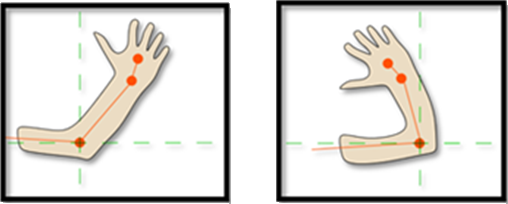
\includegraphics[width=1\textwidth]{images/wave.png}
\caption{An image from MCS UK's blog describing two parts of a wave}
\label{wave}
\end{figure}
 
They further describe this as not enough in order to accurately recognize a gesture. Stating that if the user who is waving drops his hand between the two parts, then the system would still recognize the gesture even though the actual gesture was not executed.

To resolve this problem they view the different gesture parts as different states. In figure~\ref{gesturestates} it shows three gesture parts, each resembling a state. Currently the user is in gesture part 2. There are three results, either fail, pause or succeed. Depending on certain situations these results influence the next state the system will go to.

\begin{figure}[!htbp]
\centering
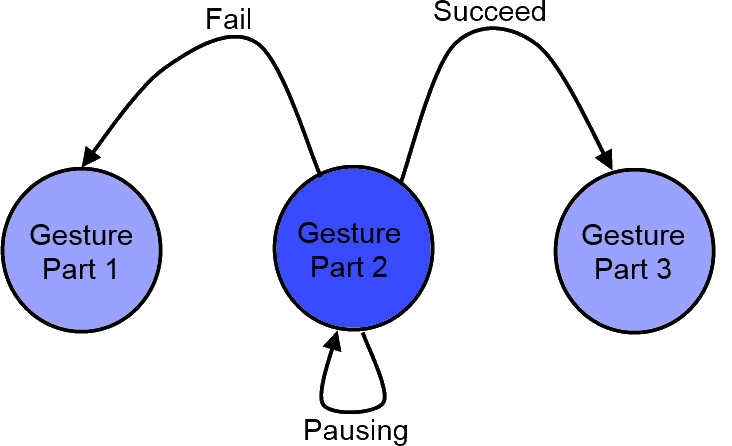
\includegraphics[width=1\textwidth]{images/gesturestate.png}
\caption{Three gesture parts resembling states}
\label{gesturestates}
\end{figure}

The fail result occurs when the user moves in an inconsistent way with the full gesture. This result will return to the begining of the gesture and start from the first gesture part. The Pausing result occurs when the user moves too slow or they did not perform the next part of the gesture. The system pauses for a maximum of 100 times. If the gesture remains and the next state was not executed then the gesture automatically fails and recognition returns from the first state again. Succeed takes place when the user executes the current part of the gesture. After a short pause the system would wait for an execution of the next gesture part from the user.

\subsubsection{Architecture of the MCS Gesture Service}
The gesture service consists of three parts. Gesture Controller, Gesture, and Gesture Parts. Figure~\ref{gestureservicearc} visualizes the architecture.

\begin{figure}[!htbp]
\centering
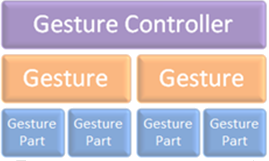
\includegraphics{images/mcsarc.png}
\caption{An image from MCS UK's blog describing the architecture of the service}
\label{gestureservicearc}
\end{figure}

The gesture controller is responsible for controlling all the gestures available for the user to perform. The gesture is responsible for controlling the gesture parts as well as keeping track of the gesture that is considered in the current state. The gesture block contains an array of IRelativeGestureSegment which are individual implementations from the IRelativeGestureSegment interface. A skeleton frame is created and checked through the states. Once the final state returs `Succeed' it raises a gesture recognized event. This event is caught by the gesture controller. The IRelativeGestureSegments resemble the individual parts of the gesture.

To handle robustness when using this method. Similar to the previous method, we take joint positions relevent to other joint points and not the axes.
\section{Connecting to the Interface}
After recognition takes place and Project Recon recognizes a gesture. Project Recon needs to send the gesture and the time frame which the gesture took place to the interface so that the interface would view it to the user in real time during practice and also keep track of his performance.

Two approaches were considered. The first focuses on using socket programming to create a server and client side where communication would occur on certain ports. The second was to use a service known as Pusher.
\subsection{Pusher \cite{citeKey4}}
Pusher is an API for creating quick realtime connection between twointernet connected devices through WebSockets.

Pusher provides many libraries for differerent frameworks like JavaScript for HTML apps or .NET and python. To better understand Pusher, figure~\ref{pusher} shows a flow diagram of Pusher.

\begin{figure}[!htbp]
\centering
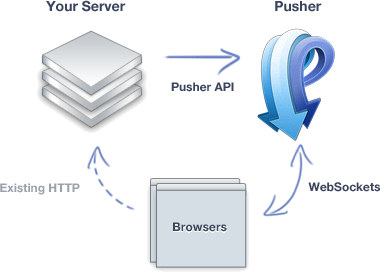
\includegraphics{images/pusher.png}
\caption{An image from Pusher's official website describing the data flow using the API}
\label{pusher}
\end{figure}

Pusher works as a Publish/Subscribe model. Where users create channels and applications connect to this channel to initiate a bi-directional connection between them.

The problem with Pusher was that it would require the user to acquire internet access at all time. Since this will not always be the case and users may be offline we will use regular socket programming.
\subsection{Socket Programming}
This approach is simple and based on the server and client connection. Where the client side will be Project Recon. This approach also helps in creating an offline connection between both applications, unlike Pusher which requires internet access on the system. From Project Recon's side we create a class, client, that will function as the link between Project Recon itself and the interface.

The class, as shown in listing~\ref{lst:client}, has four methods. One method to establish the connection, connect. The second to send data to the server, send. Finally, the method close which is responsible for closing the connection between the server and the client.

\lstinputlisting[style=csharp, caption ={Client Class},label={lst:client},float={tbp}]{listings/client.cs}

The connect method creates a new client socket and initializes a port that will be used to send the data stream to. It then aquires the IP address and creates a remote end point where to send to. Since both applications (Project Recon and the Interface), then they will both have the same IP address. After defining the remote end point we connect the socket to it.

Now that the connection is established, we send the first confirmation data. Which is a string confirming that connection is established and the Kinect is ready for inputs from the user. Before sending the data, we encode the data to bytes and call the method send and give it the new encoded data.

The method send takes three arguments two of which are the sender and the data. The method encodes the data to byte and then sends the data.

After the Kinect Sensor is connected to Project Recon, Project Recon will directly attempt to connect to the interface. Once connection is established, Project Recon will run regularly. Once a gesture or technique is recognized Project Recon will use the client method send to send a string of a certain format. The format is as shown in figure~\ref{format}.

\begin{figure}[!htb]
\centering
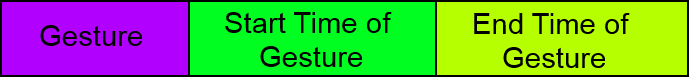
\includegraphics[width=1\textwidth]{images/format.png}
\caption{Format of the data stream sent to the interface}
\label{format}
\end{figure}

The interface will take the byte data stream and decod it to a string. It will take the time of the gesture or motion execution and from the data the interface will take certain actions.